\chapter{Super-Resolução de Imagens Pós-Inversão}
\label{cap:3modeloHibrido}

Este trabalho propõe desenvolver um novo modelo para inversão sísmica acústica e
elástica com modelagem de incerteza. No capítulo anterior foi apresentado um
método que trata o problema utilizando amostragem da distribuição posterior via
simulação sequencial direta \citep{amilcarInversao}. Outro método apresentado
utiliza o cálculo do máximo \textit{a posteriori} (MAP) para determinar o
resultado mais provável \citep{Buland01012003}.

A presente proposta tem como objetivo aumentar a eficiência do método GSI
\citep{amilcarInversao} afim de evitar amostrar soluções que não estejam dentro
da distribuição posterior. Neste caso o termo distribuição posterior é utilizado
para denotar o conjunto de soluções que é consistente com os conhecimentos
\textit{a priori} e com os dados sísmicos. Para melhorar a eficiência do método,
mantendo sua capacidade de modelagem da continuidade espacial direcional, serão
utilizadas resultados de \cite{Buland01012003} para guiar a amostragem via
imagem secundária.

Antes de efetuar a SSD, os dados de poços e resultado do MAP são submetidos à um
filtro passa alta com frequência de corte de $8Hz$. Desta forma a simulação é
efetuada somente para as frequências onde a sísmica tem amplitude significativa,
assumindo o mesmo modelo para as baixas frequências ($<8Hz$) que foi utilizado
para o cálculo do MAP. Após a simulação, o modelo de baixa frequência é
adicionado aos resultados para cálculo das sísmicas sintéticas e correlações.

O método proposto necessita dos seguintes dados de entrada: impedância acústica
medida nos poços na escala da sísmica, \textit{wavelet}, modelo de baixa
frequência para impedância acústica ($<8Hz$), matriz de covariância da sísmica,
distância de correlação vertical $L$ (Equação \ref{eq:correlVert}), modelo de
horizontes e variogramas verticais e horizontais modelados nos dados filtrados
($>8Hz$) para simulação sequencial. Resumindo, os principais passos são:


\begin{enumerate}
  \item Preparar dados de entrada e modelar variogramas
  \item Inversão pelo método MAP utilizando as matrizes de covariância da
  sísmica e do modelo, \textit{wavelet} e modelo de baixa (Equação
  \ref{eqn:mapSolution}).
  \item Filtragem dos dados de poços e resultado do MAP com filtro passa alta
  ($>8Hz$)
  \item Horizontalização dos dados de poços e resultado do MAP filtrados
  utilizando o modelo de horizontes fornecido
  \item SSD utilizando dados filtrados e horizontalizados com resultado do MAP
  como imagem secundária
  \item Reverter horizontalização das amostras simuladas pelo SSD
  \item Adicionar o modelo de baixa frequência às amostras simuladas, calcular
  refletividades e sísmica sintética. Avaliar os resultados via correlações
\end{enumerate}

O fluxo do método é ilustrado na Figura \ref{fig:fluxo}:

\begin{figure}[htp]
\begin{center}
  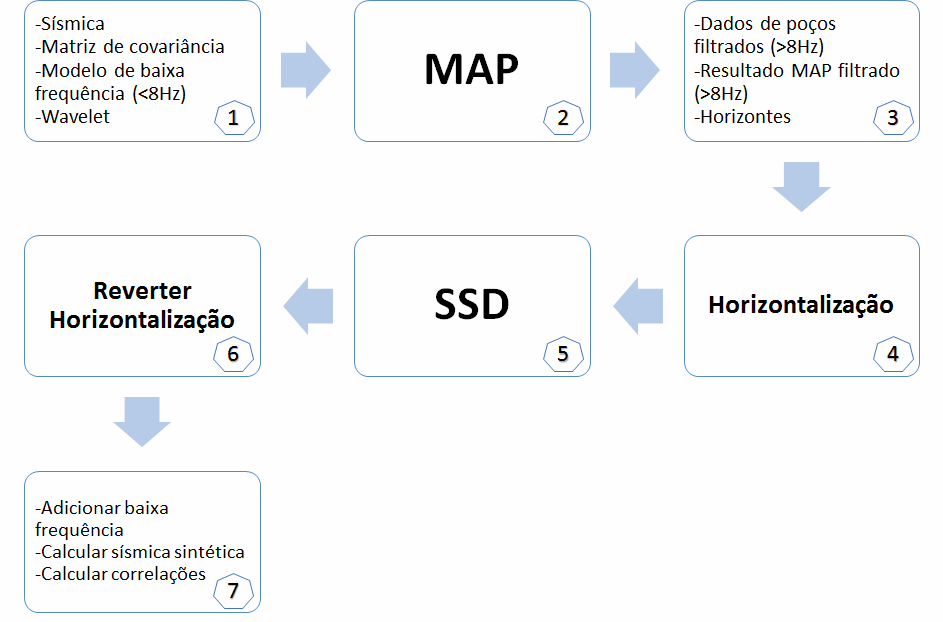
\includegraphics[width=0.6\textwidth]{fig/fluxo}
  \caption{Fluxograma do método de inversão e simulação}
  \label{fig:fluxo}
\end{center}
\end{figure}

Utilizando esta metodologia é possível gerar várias realizações da inversão para
impedância à um custo menor do que apresentado em \citep{amilcarInversao}, pois
não é mais necessário selecionar melhores amostras e efetuar iterações para
realizar a inversão, dado que o resultado do MAP já fornece uma estimativa
próxima à média desejada.


\section{Resultados Preliminares}



Experimentos realizados com o método para cálculo do MAP obtiveram resultados e
tempo de execução comparáveis com métodos implementados na indústria
\citep{leandroGRSL}. Apesar de resultar somente nas médias e variâncias, a
parametrização e regularização utilizada na metodologia pode ajudar a restringir
a amostragem, de forma a inserir informações da posterior e tornar a amostragem
do SSD mais eficiente.


Como a inversão GSI é fundamentada na Simulação Sequencial Direta, os resultados
da primeira iteração da GSI são iguais aos resultados de uma SSD utilizando os
mesmos parâmetros e dados de entrada. Desta forma é possível verificar a melhora
na correlação da sísmica sintética com a sísmica original quando se utiliza o
resultado do MAP como imagem secundária para SSD. Este experimento foi realizado
e na primeira iteração do GSI a correlação das sísmicas sintética e original foi
$0.45$ para a média de impedância, com a SSD utilizando o resultado do MAP como
imagem secundária foi obtida uma correlação de $0.97$ para a média, foram
utilizadas populações de $35$ amostras para cada método. Mesmo quando são
executadas as iterações da GSI, a máxima correlação da média encontrada é $0.9$,
tomando no mínimo 10 iterações para atingir este nível de qualidade.

Foram utilizados dados fornecidos pela PETROBRAS de um campo real para efetuar
os testes. Os dados consistem de 4 poços que se encontram na posição dos traços
17, 210, 409 e 698, modelo de baixa frequência interpolado dos poços, horizontes
e uma \textit{wavelet} extraída por um especialista da empresa. O parâmetro de
distância de correlação da inversão por MAP foi utilizado $L=1.4$, a variância da sísmica
foi estipulada como $0.4$ multiplicado pela variância média dos traços.
Para a SSD foi utlizado um modelo de variograma horizontal omnidirecional
esférico com alcance de $32$ traços, ou aproximadamente $800$ metros. Para o
variograma vertical foi utilizando o mesmo modelo com o alcance de $2$ índices
de tempo, correspondente a $8ms$.

O resultado da inversão MAP é demonstrado na Figura \ref{fig:mapResult}.
A média das realizações amostradas pelo método proposto está na Figura
\ref{fig:mapDSS}. Comparando com a Figura \ref{fig:dssresult}, a qual demonstra
a média das realizações da primeira iteração da GSI, verifica-se que utilizar o
resultado do MAP como imagem secundária traz a informação da sísmica nos pontos
entre dos poços. Comparando a média da GSI após 10 iterações, na Figura
\ref{fig:dss10result}, observa-se a semelhança dos resultados sem a necessidade
de realizar as iterações. O método proposto demorou 52s para executar contra
487s para realizar as 10 iterações da GSI.



\begin{figure}[htp]
\begin{center}
  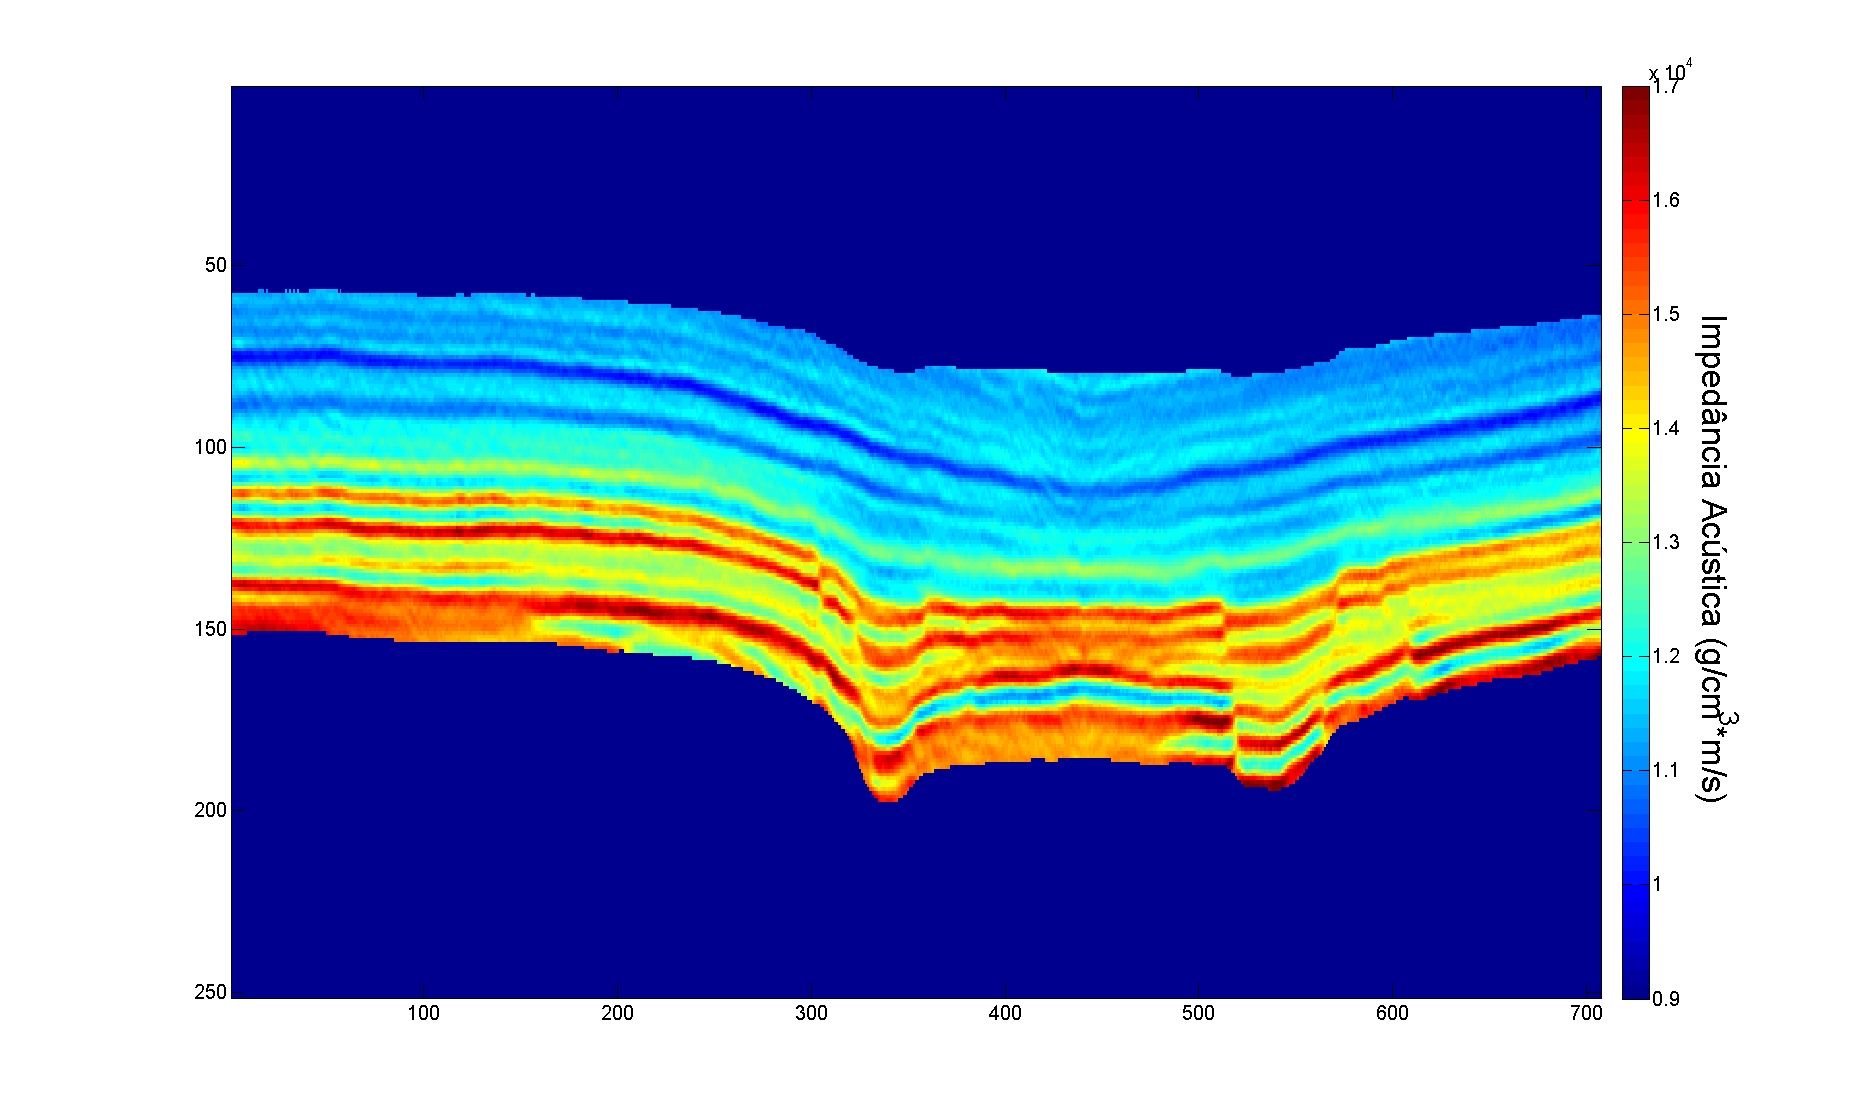
\includegraphics[width=\textwidth]{fig/map}
  \caption{Resultado MAP utilizado como imagem secundária}
  \label{fig:mapResult}
\end{center}
\end{figure}


\begin{figure}[htp]
\begin{center}
  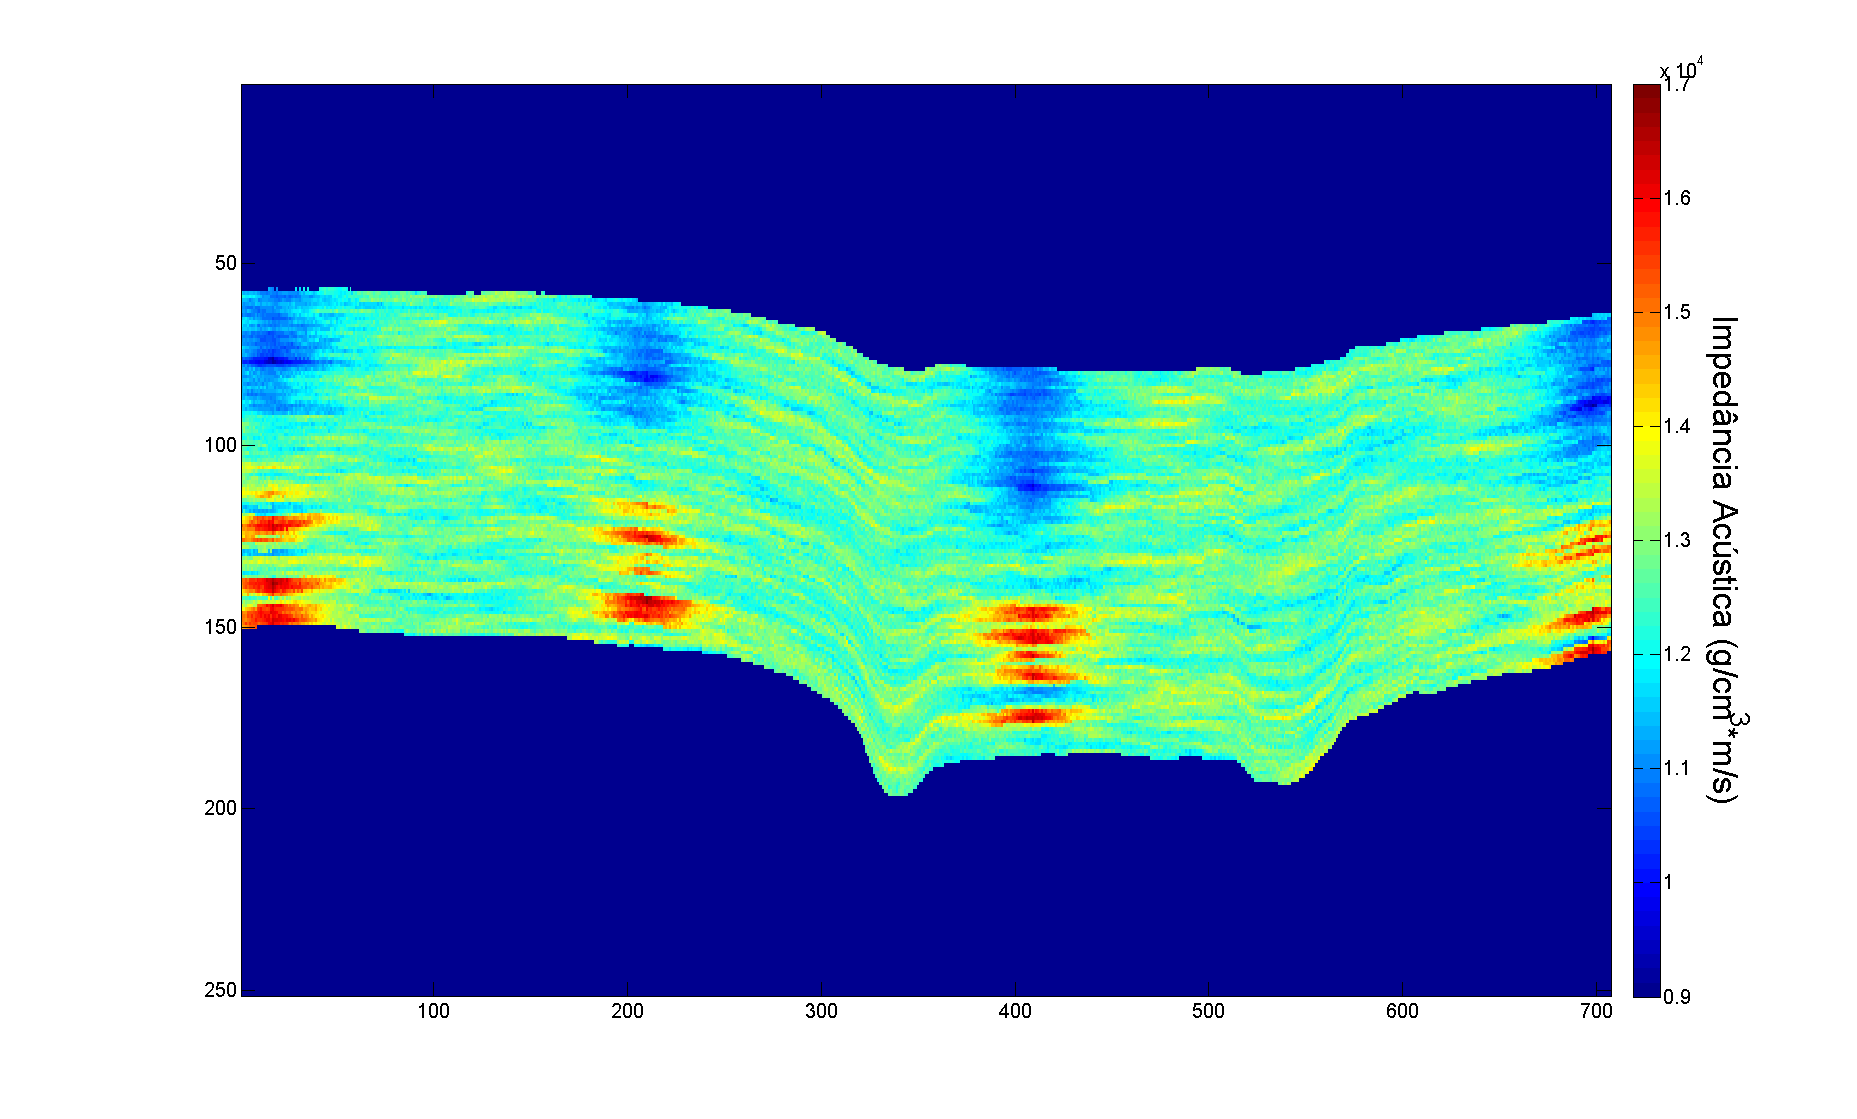
\includegraphics[width=\textwidth]{fig/dss1it-20realz}
  \caption{Média das amostras da primeira iteração da GSI}
  \label{fig:dssresult}
\end{center}
\end{figure}

\begin{figure}[htp]
\begin{center}
  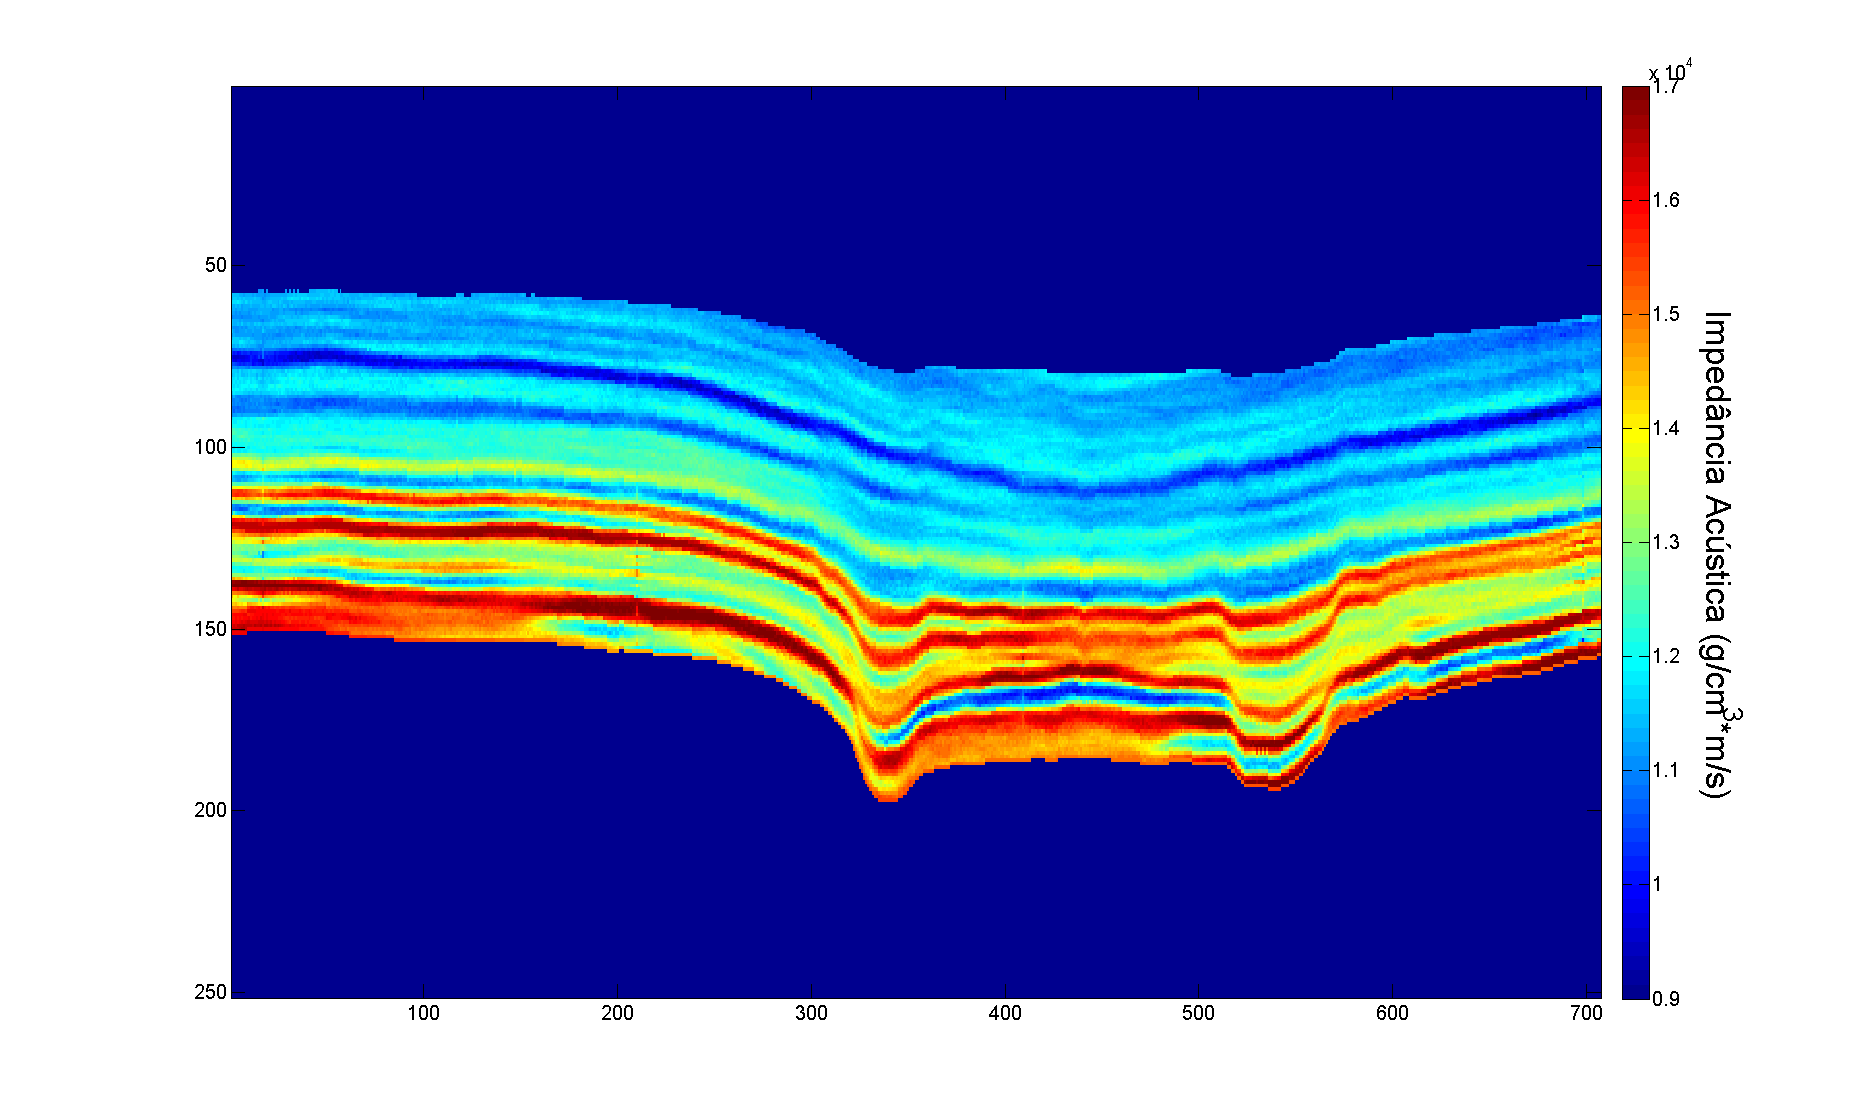
\includegraphics[width=\textwidth]{fig/mapdss1it-20realz-filt}
  \caption{Média das amostras da SSD utilizando MAP como imagem
  secundária}
  \label{fig:mapDSS}
\end{center}
\end{figure}


\begin{figure}[htp]
\begin{center}
  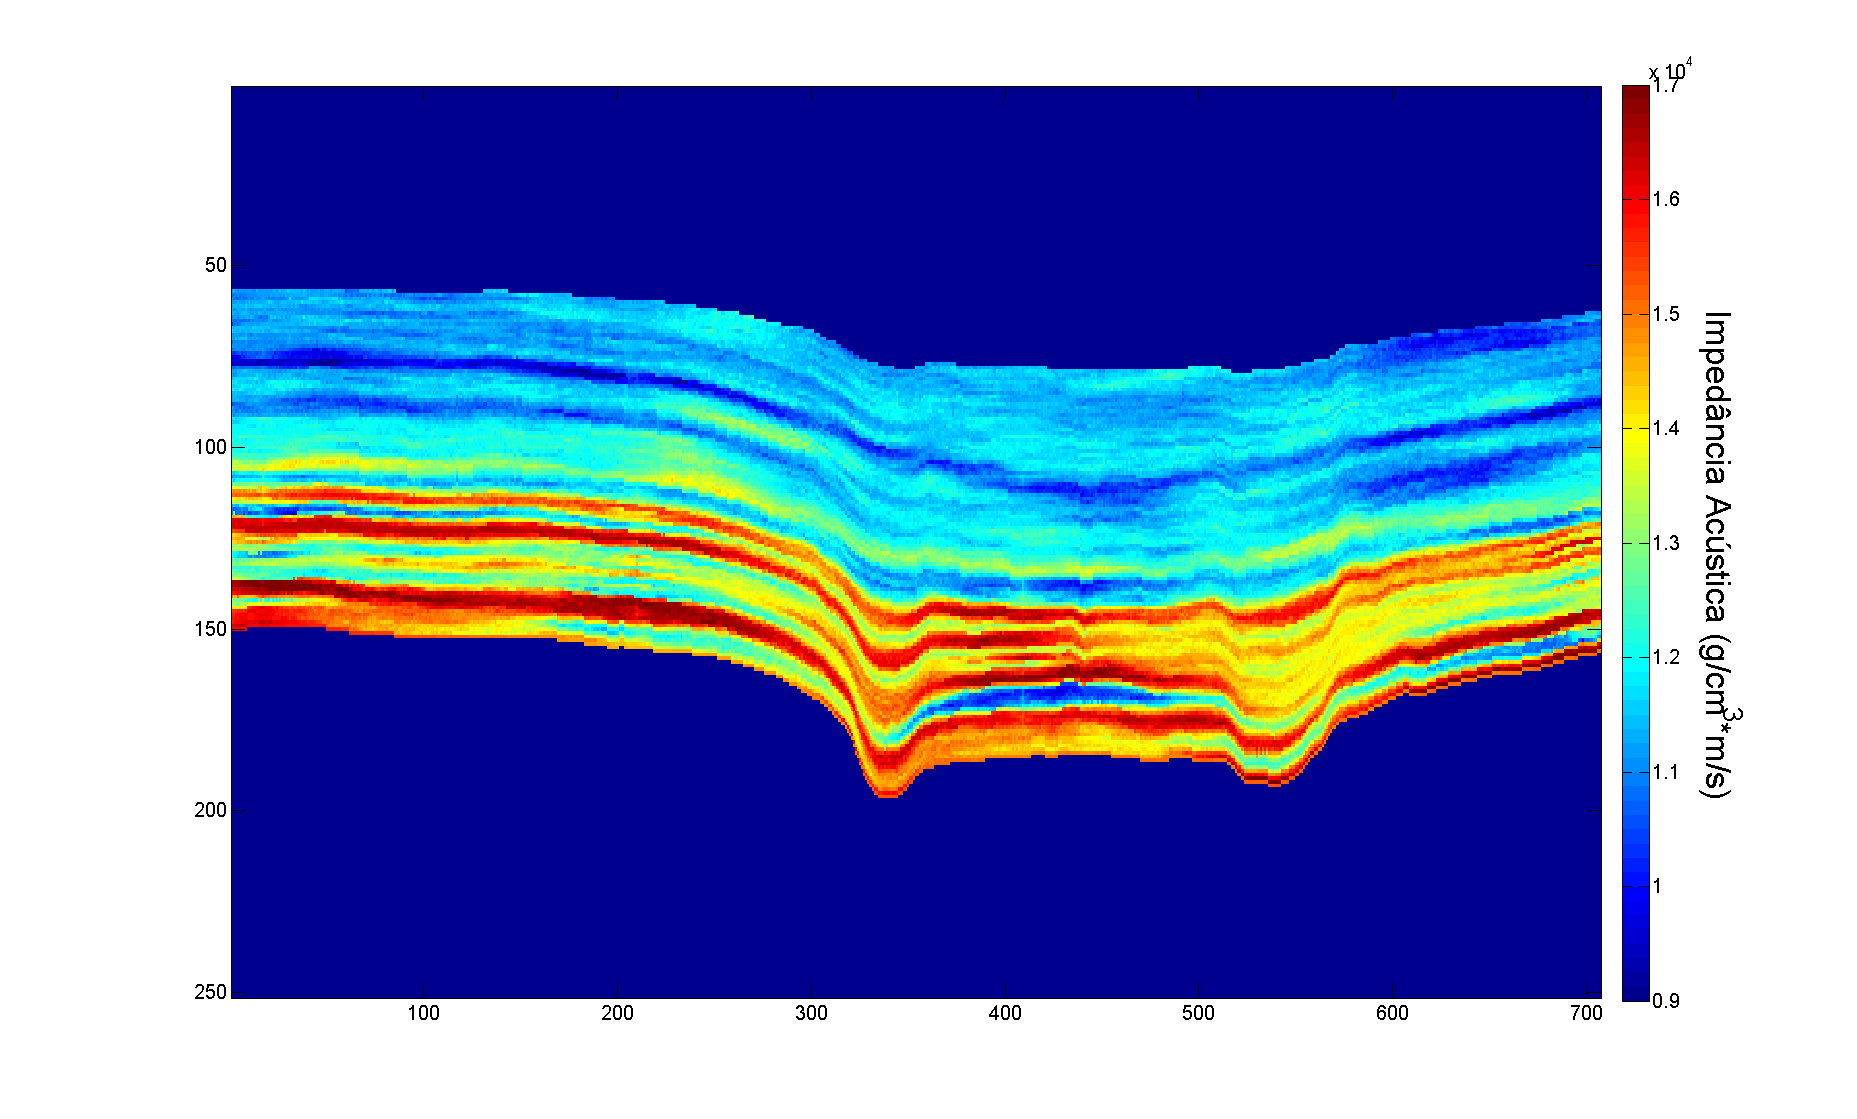
\includegraphics[width=\textwidth]{fig/dss10it-20realz}
  \caption{Média das amostras após 10 iterações da GSI}
  \label{fig:dss10result}
\end{center}
\end{figure}

A metodologia descrita na literatura para a GSI não aplica a filtragem dos dados
para amostrar somente os resíduos, ou alta frequência. Utilizar o modelo de
baixa frequência como informação \textit{a priori} foi identificado como uma
regularização importante para agilizar a inversão e amostragem. Principalmente
para a SSD, filtrar os dados resulta em uma distribuição global com menor
variância, pois assumindo um modelo de baixa frequência são definidas médias
locais e as amostras são geradas em torno desta média, respeitando a
distribuição do poço filtrado. Sem a filtragem, a informação da média local não
é utilizada, amostrando-se toda a distribuição original do poço em todos os
pontos da região de interesse. A Figura \ref{fig:pocoFilteN} mostra a comparação
dos histogramas dos dados filtrados e não filtrados. Portanto, utilizar o modelo
de baixa frequência insere um viés no resultado e diminui a incerteza dada pela
variância, mas a incerteza referente a escolha do modelo de baixa precisa ser
levada em consideração.


\begin{figure}
        \centering
        \begin{subfigure}[b]{0.45\textwidth}
                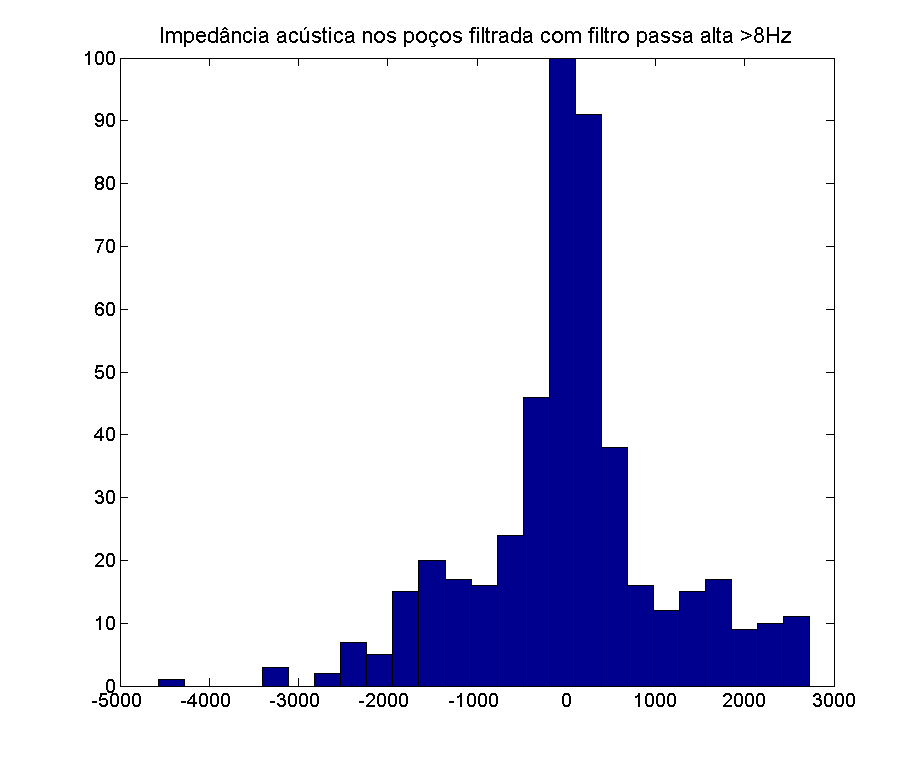
\includegraphics[width=\textwidth]{fig/IA_com_filtro}
                \caption{Dados filtrados}
        \end{subfigure}%
        \hfill
        \begin{subfigure}[b]{0.45\textwidth}
                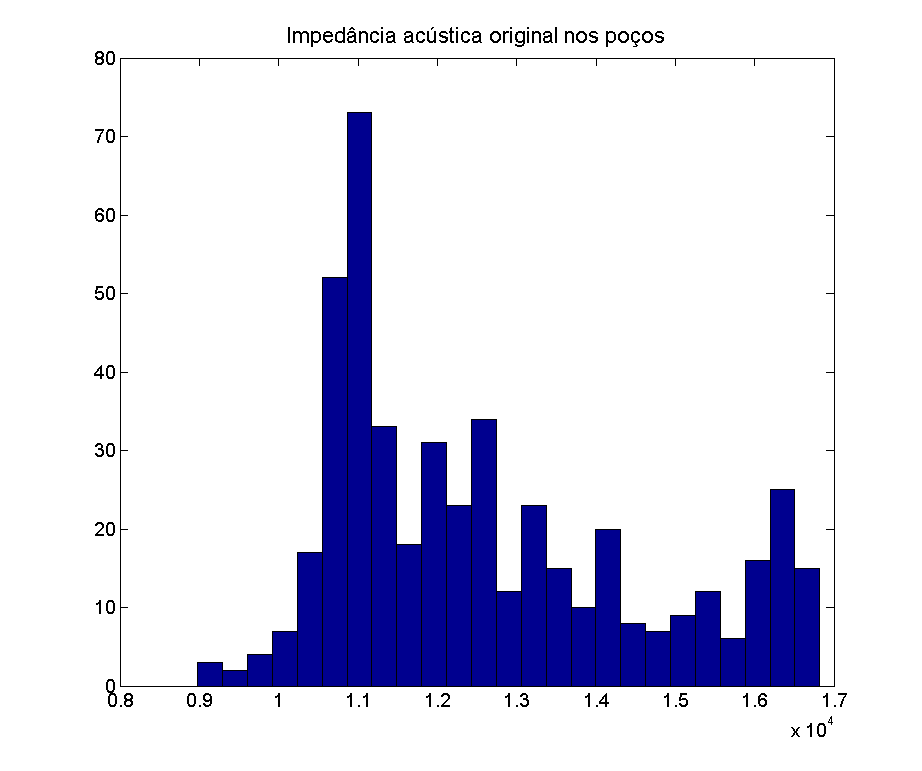
\includegraphics[width=\textwidth]{fig/IA_sem_filtro}
                \caption{Dados originais}
        \end{subfigure}
        \caption{Comparação dos dados de poços filtrados}\label{fig:pocoFilteN}
\end{figure}





\section{Proposta e Plano de Trabalho}

A proposta para o restante do projeto é implementar a inversão elástica, que
utiliza sísmica pré empilhada para obter as velocidades primária e secundária e
densidade na linha de \cite{azevedo2013_avoinv} dentro da nova metodologia
proposta. Os resultados obtidos serão comparados com os resultados da GSI em
termos de variância e qualidade do resultado baseado na metodologia de
\cite{coleou_qualityanomalyinv}, amplamente utilizada para avaliação dos
resultados da inversão sísmica na indústria.

A metodologia de \cite{caers_distance_kernels_MDS} será integrada na proposta
para possibilitar a análise da incerteza envolvida com os parâmetros e dados de
entrada definidos pelo especialista, como o modelo de baixa, \textit{wavelets} e
horizontes, pois a essas incertezas geológicas são apontadas como maiores
influências na incerteza do resultado da inversão \citep[p.
133]{caers2011modeling}. Para tanto, será proposto um esquema de amostragem com
Monte Carlo para selecionar os dados de entrada aleatoriamente a cada amostragem
do resultado da inversão. Após obter várias amostras com combinações diferentes
de dados de entrada, uma análise baseada em \textit{Multi-Dimensional Scaling}
será aplicada para avaliar a sensibilidade ao variar cada parâmetro de entrada
na incerteza final do resultado da inversão. Será utilizada como métrica as
medidas de \textit{Quality-Anomaly} \citep{coleou_qualityanomalyinv}.

O caráter de originalidade do trabalho é garantido pelas contribuições para a
área de inversão com modelagem de incerteza. A primeira contribuição diminui o
tempo de execução por eliminar a necessidade de um método iterativo para
realizar a inversão geoestatística, ao mesmo tempo modelando a continuidade
lateral. A segunda contribuição será modelar as incertezas presentes nos dados
de entrada (\textit{wavelets}, horizontes, modelos de baixa, variogramas,
etc\ldots) após a integração da metodologia de
\cite{caers_distance_kernels_MDS}.

A Figura \ref{fig:gantt} mostra o cronograma mensal das atividades a serem
desenvolvidas durante o período de 12 meses do estágio de doutorado sanduíche a
ser realizado no Centro de Recursos Naturais e Ambiente (CERENA) do Instituto
Superior Técnico (IST) ligado a Universidade de Lisboa sob orientação do Dr.
Amilcar Soares. Também estão planejados os meses após o retorno para finalização
da tese e defesa.


\begin{figure}[htp]
\begin{center}
  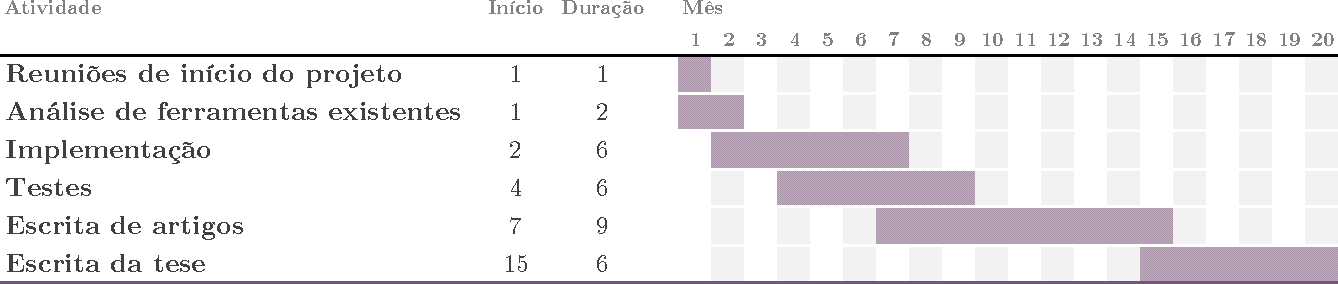
\includegraphics[width=\textwidth]{fig/gantt_EQD}
  \caption{Cronograma mensal do projeto a partir de jul/2014}
  \label{fig:gantt}
\end{center}
\end{figure}

Dentre os periódicos que apresentam trabalhos relacionados com esta área, se
destacam os seguintes com suas classificações no Qualis para Ciências da
Computação:

\begin{itemize}
  \setlength{\itemsep}{0pt}
  \setlength{\parskip}{0pt}
  \item IEEE Trans. on Geoscience and Remote Sensing
  \item ISSN: 0196-2892 - IEEE - Qualis A1
\end{itemize}

\begin{itemize}
  \setlength{\itemsep}{0pt}
  \setlength{\parskip}{0pt}
  \item Journal of Computational Physics
  \item ISSN: 0021-9991 - Elsevier - Qualis A1
\end{itemize}

\begin{itemize}
  \setlength{\itemsep}{0pt}
  \setlength{\parskip}{0pt}
  \item Computers \& Geosciences
  \item ISSN: 0098-3004 - Elsevier - Qualis A2
\end{itemize}


\begin{itemize}
  \setlength{\itemsep}{0pt}
  \setlength{\parskip}{0pt}
  \item Computational Geosciences
  \item ISSN: 1420-0597 - Springer - Qualis B1
\end{itemize}


\begin{itemize}
  \setlength{\itemsep}{0pt}
  \setlength{\parskip}{0pt}
  \item Geophysics
  \item ISSN: 0016-8033 - Society of Exploration Geophysicists - Qualis A2 Interdisciplinar
\end{itemize}


\begin{itemize}
  \setlength{\itemsep}{0pt}
  \setlength{\parskip}{0pt}
  \item Mathematical Geosciences
  \item ISSN: 1874-8961 - Springer - Qualis A2 Interdisciplinar
\end{itemize}


A colaboração com o grupo de pesquisas do Prof. Amilcar Soares é justificada
pois o autor é a uma das principais referências na literatura sobre Simulação
Sequencial Direta e inversão Geoestatística
\citep{azevedo2013_avoinv,amilcarInversao,2001amilcarDSS}. A pesquisa nos dois
primeiros anos do projeto de Doutorado foi feita sob orientação do Prof. Mauro
Roisenberg, coautor de referências relevantes para inversão Bayesiana
\citep{leandro_SEG,leandroGRSL}. Desta forma, espera-se cumprir a proposta de
integração sob orientação de especialistas em ambos os métodos. A proposta
também faz parte de um Termo de Cooperação Petrobras/UFSC/FEESC.


